\documentclass[12pt]{report}
\usepackage[english]{babel}
\usepackage[utf8]{inputenc}
\usepackage[hyphens]{url}
\usepackage{titlesec, float, graphicx}
\usepackage{enumitem}
\usepackage{graphicx}
\usepackage{listings}
\usepackage{amsmath}
\usepackage{xcolor}
\usepackage{courier}
\usepackage{amsmath}
\usepackage[final]{pdfpages}
\usepackage{caption}
\usepackage{subcaption} 
\usepackage{pdfpages}
\usepackage[unicode]{hyperref}

\newcommand\tab[1][1cm]{\hspace*{#1}}
\titleformat{\chapter}{\normalfont\huge}{\thechapter.}{20pt}{\huge}
\lstset{
	language=Java, 
	frame=single,
    breaklines=true,
    basicstyle=\ttfamily
    % postbreak=\mbox{\textcolor{red}{$\hookrightarrow$}\space}
    }
\begin{document}
%
% Zacatek titulni strany
%
\pagenumbering{gobble} 
\begin{center}

\includegraphics[scale=0.2]{img/ulpgc_logo.jpg}
\vspace{5cm}\linebreak
\Huge{Design of user interfaces}\linebreak
\large{Square matrix filtration}\linebreak
\normalsize{2018/19 course - Practice 1}\linebreak
\vspace{3cm}\linebreak

\small{David Bohmann}\linebreak
\small{Petr Lukašík}\linebreak
\today\linebreak
\end{center}
%
% Konec titulni strany
%

%
% Obsah
%
\newpage
{\footnotesize \tableofcontents}

%
% Zadání
%

\chapter{Assigment}
\label{chap:assig}
\pagenumbering{arabic}
The objective of this practice is to introduce the panels as well as the components of the slide bar and text area. The application should show in an area of text the elements of a square matrix of dimension 10x10 that exceed the value selected by the slide bar.
\\ \\
This application should allow the user:
\begin{itemize}
\item Enter the maximum and minimum values contained in the matrix of whole.
\item Show the square matrix in a text area with integer values generated randomly between the maximum and minimum values introduced.
\item Include a sliding bar with marks and labels of values that allow to dynamically select the threshold. All the elements of the matrix with value less than or equal to that indicated on the slide bar is will show as a script (-) in the text area.
\end{itemize}
\\
It should be noted that:
\begin{itemize}
    \item The elements that must be separated in two different panels configure the result of the text area where the matrix is shown filtered.
    \item No button will be available to start processing.
    \item Any change in dimension, maximum or minimum value supposes initialize and show the new matrix.
    \item Changes in the threshold using the slide bar only will involve filtering the lower values and updating the area of text.
    \item Documentation to be delivered
\end{itemize}
%
% Uvod
%
\chapter{Implementation}
For programming we used Netbeans IDE with Java 8. We have programmed an application which is creating matrix based on inputs of matrix dimension, minimum matrix value and maximum matrix value as seen in \ref{fig:inputs}. Under input textboxes is placed threshold slider shown in figure \ref{fig:slider}, which dynamically shows "-" for any number in matrix lower or equal than threshold value. For better user friendly environment we even created error label on figure \ref{fig:errlabel}, that shows error messages when user inputs incorrect format inside textboxes (e.g. not integer). In the bottom part of application is located textarea shown in \ref{fig:app} for the output matrix.
\begin{figure}[!ht]
\centering
\begin{subfigure}{\textwidth} 
  \centering
  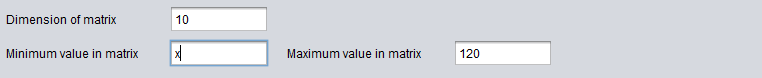
\includegraphics[width=\linewidth]{img/inputs.PNG}
  \caption{Detail on inputs}
  \label{fig:inputs}
\end{subfigure}
\begin{subfigure}{\textwidth}
  \centering
  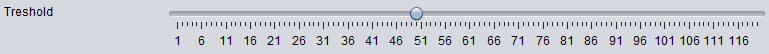
\includegraphics[width=\linewidth]{img/threshold.PNG}
  \caption{Detail on slider}
  \label{fig:slider}
\end{subfigure}
\begin{subfigure}{\textwidth}
  \centering
  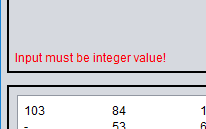
\includegraphics[height=3cm, keepaspectratio]{img/errlabel.PNG}
  \caption{Detail on error label}
  \label{fig:errlabel}
\end{subfigure}
\caption{Single components in the application}
\label{fig:compview}
\end{figure}
\\
Whole application was tested many times to eliminate all exceptions in the program. The main concept was followed to the detail and it should be working perfectly.

\begin{figure}[!ht]
\centering
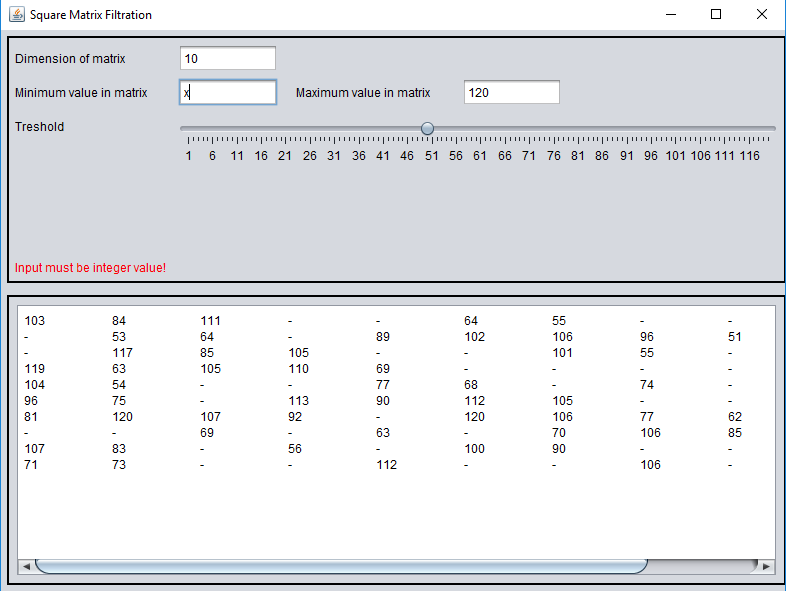
\includegraphics[width=.8\linewidth]{img/application.PNG}
\caption{Our square matrix filtration application}
\label{fig:app}
\end{figure}

\chapter{Shneiderman and Plaisant principles}
\begin{itemize}
    \item \textbf{Consistency} \\
    Since we are creating only one application window there is not much space to be consistent at design. Window should be intuitive, upper half is for settings, bottom half is for displaying result.
    \item \textbf{Universal usability} \\
    For the purpose this application is created the usability of this application is pretty straight. There is almost nothing that user can do except of changing values of inputs. All inputs are executed instantly.  
    \item \textbf{Informative feedback} \\
    If user writes wrong data into input textboxes, the error label automatically popup to show what is wrong with inputs. If input data are good, when changing, the textarea instantly shows result.
    \item \textbf{Design dialogue to yield closure} \\
    If every input is right, changing inputs displays results instantly in bottom textarea.
    \item \textbf{Simple error handling.} \\
    Implemented error label is in the bottom of settings to tell you what is wrong.
    \item \textbf{Permit easy reversal of actions} \\
    This is something we didn't implement in our application. There is no possibility to reverse current action.
    \item \textbf{Support internal locus of control} \\
    The user should be in full control of how big matrix and the dispersion of numbers he wants to create and what threshold to set for matrix values. 
    \item \textbf{Reduce short-term memory load} \\
    This is hard to say for such a small application, but from a big perspective our application is fast enough for human needs.
\end{itemize}
\end{document}